%%%%%%%%%%%%%%%%%%%%%%%%%%%%%%%%%%%%%%%%%%%%%%%%%%%%%%%%%%%%%%%%%%%%%
%%%%%%%%%%%%%%%%%%%%%%%%%%%%%%%%%%%%%%%%%%%%%%%%%%%%%%%%%%%%%%%%%%%%%
%%%%%%%%%%%%%%%%%%%%%%%%%%%%%%%%%%%%%%%%%%%%%%%%%%%%%%%%%%%%%%%%%%%%%
\section{Further comments and examples}\label{sec:comments_and_examples}

In this last section we compile a few comments related to \cite{FPST} and provide an example further illustrating the techniques developed in Sections \ref{sec:graded-QP}, \ref{sec:euler}, \ref{sec:dilation_plabic_fence} and \ref{sec:polynomial_plabic_fence}.

%%%%%%%%%%%%%%%%%%%%%%%%%%%%%%%%%%%%%%%%%%%%%%%%%%%%%%%%%%%%%%%%%%%%%
%%%%%%%%%%%%%%%%%%%%%%%%%%%%%%%%%%%%%%%%%%%%%%%%%%%%%%%%%%%%%%%%%%%%%
\subsection{A counterexample to \cite[Conjecture 6.17]{FPST}} The article \cite{FPST} contains other interesting conjectures. For instance, it is proven in \cite[Proposition 6.16]{FPST} that if two plabic graphs are move-and-switch equivalent to each other, then their associated quivers are mutation equivalent. It is then stated in \cite[Conjecture 6.17]{FPST} that it is conjectured to be an equivalence, i.e.~that two plabic graphs are move-and-switch equivalent if and only if their associated quivers are mutation equivalent.\\


\begin{figure}
\centering
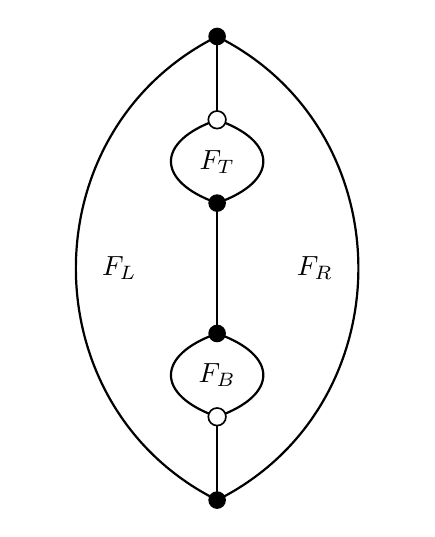
\begin{tikzpicture}[scale=.92,
  bvertex/.style={circle,fill=black,inner sep=2.25pt},
  wvertex/.style={circle,fill=white,draw=black,line width=.6pt,inner sep=2.25pt},
  every path/.style={line width=.8pt}]
\coordinate (v0) at (0,3.2);
\coordinate (v1) at (0,2.05);
\coordinate (v2) at (0,.9);
\coordinate (v3) at (0,-.9);
\coordinate (v4) at (0,-2.05);
\coordinate (v5) at (0,-3.2);
\draw (v0) .. controls (-2.6,1.9) and (-2.6,-1.9) .. (v5);
\draw (v0) .. controls (2.6,1.9) and (2.6,-1.9) .. (v5);
\draw (v0)--(v1);
\draw (v1) .. controls (-.85,1.75) and (-.85,1.2) .. (v2);
\draw (v1) .. controls (.85,1.75) and (.85,1.2) .. (v2);
\draw (v2)--(v3);
\draw (v3) .. controls (-.85,-1.2) and (-.85,-1.75) .. (v4);
\draw (v3) .. controls (.85,-1.2) and (.85,-1.75) .. (v4);
\draw (v4)--(v5);
\node[bvertex] at (v0) {};
\node[wvertex] at (v1) {};
\node[bvertex] at (v2) {};
\node[bvertex] at (v3) {};
\node[wvertex] at (v4) {};
\node[bvertex] at (v5) {};
\node at (-1.35,0) {$F_L$};
\node at (1.35,0) {$F_R$};
\node at (0,1.47) {$F_T$};
\node at (0,-1.47) {$F_B$};
\end{tikzpicture}\qquad\qquad
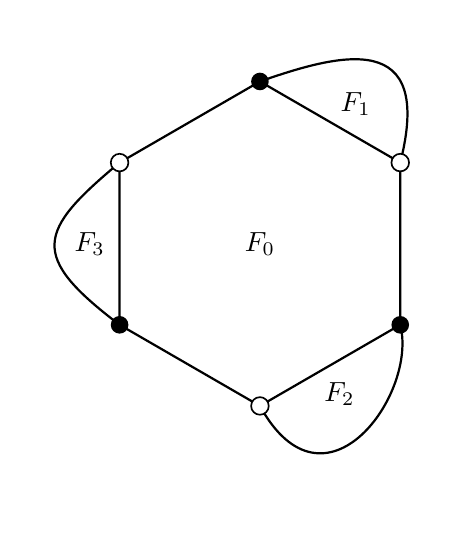
\begin{tikzpicture}[scale=1.03,
  bvertex/.style={circle,fill=black,inner sep=2.25pt},
  wvertex/.style={circle,fill=white,draw=black,line width=.6pt,inner sep=2.25pt},
  every path/.style={line width=.8pt}]
\coordinate (u1) at (0,2);
\coordinate (u2) at (1.73,1);
\coordinate (u3) at (1.73,-1);
\coordinate (u4) at (0,-2);
\coordinate (u5) at (-1.73,-1);
\coordinate (u6) at (-1.73,1);
\draw (u1)--(u2)--(u3)--(u4)--(u5)--(u6)--cycle;
\draw (u1) .. controls (1.0,2.35) and (2.15,2.65) .. (u2);
\draw (u3) .. controls (1.95,-1.85) and (.8,-3.45) .. (u4);
\draw (u5) .. controls (-2.85,-.15) and (-2.75,.15) .. (u6);
\node[bvertex] at (u1) {};
\node[wvertex] at (u2) {};
\node[bvertex] at (u3) {};
\node[wvertex] at (u4) {};
\node[bvertex] at (u5) {};
\node[wvertex] at (u6) {};
\node at (0,0) {$F_0$};
\node at (1.18,1.72) {$F_1$};
\node at (.98,-1.85) {$F_2$};
\node at (-2.1,0) {$F_3$};
\end{tikzpicture}
\caption{Two plabic graphs, $G_0$ on the left, and $G_1$ on the right.}
\label{fig:plabic_graphs_Shapiro}
\end{figure}


Consider the two plabic graphs in \Cref{fig:plabic_graphs_Shapiro}. The plabic graph $G_0$ in \Cref{fig:plabic_graphs_Shapiro} (left) is the one drawn in \cite[Figure 8.(b)]{GL}. The corresponding quivers $Q(G_0)$ and $Q(G_1)$ are

\[
Q(G_0)\;=\;
\begin{tikzcd}[row sep=3.2em,column sep=3.8em]
F_T \arrow[r] & F_R \arrow[d] \\
F_L \arrow[u] & F_B \arrow[l]
\end{tikzcd}
\quad\quad\&\quad\quad
Q(G_1)\;=\;
\begin{tikzcd}[row sep=3.2em,column sep=3.8em]
F_1 \arrow[dr] & & F_2 \arrow[dl] \\
& F_0 & \\
& F_3 \arrow[u] &
\end{tikzcd}
\]
Note that $Q(G_1)$ is an orientation of the $D_4$-Dynkin diagram. By mutating $Q(G_0)$ first at $F_T$ and then at $F_R$ and $F_L$, say, it follows that $Q(G_0)$ is mutation equivalent to $Q(G_1)$.\\

Now, for a plabic graph $\mathbb{P}$, the local moves in \cite[Definition 6.2]{FPST} preserve the smooth type of the associated link $L(\mathbb{P})$.\footnote{See \cite[Section 9]{FPST} for the definition of $L(\mathbb{P})$. In brief, it is the smooth link obtained by satelliting along the unknot the Legendrian link in the unit cotangent bundle of the plane whose front projection is the alternating strand diagram of the plabic graph.} In contrast, the switch operation on a plabic graph $\mathbb{P}$, as defined in \cite[Definition 6.15]{FPST}, has the effect of changing the associated link $L(\mathbb{P})$ by a positive Conway mutation. See \cite{Conway1970} and \cite[Section~1]{Morton2015} for the notion of a tangle mutation. Now, by \cite[Statement~11]{Hoste1986}, the HOMFLY polynomial of a link is invariant under positive Conway
mutation, see also \cite[Proposition~11]{LickorishMillett1987} and ~\cite{FreydEtAl1985}. In particular, \cite[Conjecture 9.6]{GL} is true. Therefore, if $G_0$ and $G_1$ were move-and-switch equivalent, their links $L(G_0)$ and $L(G_1)$ would have identical HOMFLY polynomials.\\

For $G_0$, the associated HOMFLY polynomial of the plabic link is computed explicitly \cite[Section~9.3]{GL}:
\begin{equation}\label{eq:P0}
\begin{aligned}
\HOMFLY(L(G_0);a,z)
={}&a^{-4}(z^4+4z^2+2)+a^{-8}z^{-2}-a^{-10}(z^2+3+2z^{-2})
+a^{-12}(1+z^{-2}).
\end{aligned}
\end{equation}

\noindent Here $\HOMFLY(L;a,z)$ denotes the oriented HOMFLY polynomial normalized by
\begin{equation}\label{eq:homfly-skein}
a\HOMFLY(L_+;a,z)-a^{-1}\HOMFLY(L_-;a,z)=z\HOMFLY(L_0;a,z),
\qquad
\HOMFLY(\bigcirc;a,z)=1.
\end{equation}

\noindent To compute the HOMFLY polynomial associated to $G_1$ we use \cite{Schwartz}, as $G_1$ is simple. Specifically, \cite[Theorem~3.11]{Schwartz} shows that, for a connected plabic graph whose face quiver is a forest, the HOMFLY polynomial of the plabic link is the forest-quiver polynomial. Note that this polynomial depends only on the underlying unoriented forest, which in our case is a $D_4$-Dynkin diagram. Therefore \cite[Example~4.8]{Schwartz} yields
\begin{equation}\label{eq:P1}
\begin{aligned}
\HOMFLY(L(G_1);a,z)
={}&a^{-4}(z^4+4z^2+3+z^{-2})-a^{-6}(z^2+3+2z^{-2})
+a^{-8}z^{-2}.
\end{aligned}
\end{equation}

\noindent Since the coefficient of $a^{-6}$ in \eqref{eq:P1} is non-zero, and it is zero in \eqref{eq:P0}, these two HOMFLY polynomials are distinct. Thus $G_0$ and $G_1$ are not move-and-switch equivalent. We conclude that it is possible for two plabic graphs to have mutation equivalent quivers while not being move-and-switch equivalent, contradicting \cite[Conjecture 6.17]{FPST}.
%%%%%%%%%%%%%%%%%%%%%%%%%%%%%%%%%%%%%%%%%%%%%%%%%%%%%%%%%%%%%%%%%%%%%
%%%%%%%%%%%%%%%%%%%%%%%%%%%%%%%%%%%%%%%%%%%%%%%%%%%%%%%%%%%%%%%%%%%%%

\subsection{A detailed example}\label{ssec:examples}

Let us consider the irreducible isolated plane curve singularity
\[
 C:=\{(x,y)\in\C^2:x^3-y^4=0\}.
\]
The singularity is at the origin $(x,y)=(0,0)$: it is the $E_6$ simple singularity and its link is the $(3,4)$-torus knot. See also \cite[Figure 4]{FPST} for two divides associated to two real Morsifications of this singularity. Let us consider the top divide for $E_6$ in \cite[Figure 4]{FPST}. Its associated quiver $Q$ is

\[
\begin{tikzcd}[column sep=large, row sep=large]
1
  \arrow[r, "a"]
  \arrow[d, "e"']
&
2
  \arrow[r, "b"]
  \arrow[d, "f"']
&
3
  \arrow[d, "g"]
\\
4
  \arrow[r, "c"']
&
5
  \arrow[r, "d"']
  \arrow[ul, "p"]
&
6
  \arrow[ul, "q"]
\end{tikzcd}
\]
\noindent The associated non-degenerate potential is
\begin{equation}\label{eq:E6-W}
 W=pfa-pce+qgb-qdf.
\end{equation}
An arrow-grading $d:Q_1\lr\Z$ for which $W$ in \eqref{eq:E6-W} is homogeneous of degree 1 is
\begin{equation}\label{eq:E6-d}
 d(p)=d(q)=1,
 \qquad
 d(a)=d(b)=d(c)=d(d)=d(e)=d(f)=d(g)=0.
\end{equation}

Consider the bigraded Ginzburg dg algebra $\Gamma(Q,W,d)$ as in \Cref{def:bigradedGinzburg} and the derived category $\D^{\gr}_{\fd}(\Gamma)$ as in \Cref{def:categories_over_bigraded}. The graded Euler pairing expressed in the simple basis reads
\begin{equation}\label{eq:E6-E}
 \Eul_{Q,W,d}(t)=
 \begin{pmatrix}
 1-t&-1&0&-1&1&0\\
 t&1-t&-1&0&-1&1\\
 0&t&1-t&0&0&-1\\
 t&0&0&1-t&-1&0\\
 -t&t&0&t&1-t&-1\\
 0&-t&t&0&t&1-t
 \end{pmatrix},
\end{equation}
which can be computed directly or via \Cref{prop:euler-formula}. In particular, its determinant is
\begin{equation}\label{eq:E6-det}
 \det\Eul_{Q,W,d}(t)
 =(t^2-t+1)(t^4-t^2+1)
 =t^6-t^5+t^3-t+1.
\end{equation}
Note that \eqref{eq:E6-det} coincides with the Alexander polynomial $\Delta_{T(3,4)}(t)$ of the $(3,4)$-torus knot, in accordance with \Cref{cor:cokernel_module_is_Alexander_algebraic_links}.\\

Let us now mutate the quiver $Q$ at the vertex $1$. The only incoming arrow is \(p:5\to1\), and there are two outgoing arrows \(a:1\to2\) and \(e:1\to4\). In order to perform the QP mutation of $(Q,W)$, introduce the composite arrows
\[
 x=[ap]:5\to2,\qquad y=[ep]:5\to4,
\]
and reversed arrows
\[
 \alpha=a^*:2\to1,\qquad
 \varepsilon=e^*:4\to1,\qquad
 \pi=p^*:1\to5.
\]
Then the premutated potential is cyclically equivalent to
\begin{equation}\label{eq:E6-premut}
 \widetilde W=xf-yc+qgb-qdf+\pi\alpha x+\pi\varepsilon y.
\end{equation}
Now we need to extract the reduced part. For that let us set
\[
 x_0:=x-qd,\qquad c_0:=c-\pi\varepsilon,
 \qquad f_0:=f+\pi\alpha.
\]
Then we obtain the cyclic equivalence
\[
 \widetilde W\sim_{\cyc}
 x_0f_0-yc_0+qgb+\pi\alpha qd,
\]
so that $x_0f_0$ and $yc_0$ are trivial pairs. After deleting these two trivial pairs, the quiver $Q'$ for the reduced QP $(Q',W')$ reads
\[
\begin{tikzcd}[column sep=large, row sep=large]
1
  \arrow[dr, "\pi"]
&
2
  \arrow[l, "\alpha"']
  \arrow[r, "b"]
&
3
  \arrow[d, "g"]
\\
4
  \arrow[u, "\varepsilon"]
&
5
  \arrow[r, "d"']
&
6
  \arrow[ul, "q"']
\end{tikzcd}
\]
and the corresponding potential $W'$ reads
\begin{equation}\label{eq:E6-mut-W}
 W'=qgb+\pi\alpha qd.
\end{equation}
The corresponding mutated grading is
\begin{equation}\label{eq:E6-mut-d}
 d'(q)=1,\qquad d'(u)=0\quad(u\ne q),
\end{equation}
which indeed makes $W'$ homogeneous of degree one. Note that $Q'$ is {\it not} the quiver associated to any divide, as the 4-cycle $\pi\alpha qd$ would violate the rule $\bullet\to\oplus\to\ominus\to\bullet$ in \cite[Definition 4.2]{FPST}. This illustrates that quiver mutation typically forces one out of the class of quivers with divides. This is what makes the Main Conjecture challenging. Finally, the graded Euler pairing for $(Q',W',d')$ in the simple basis reads
\begin{equation}\label{eq:E6-mut-E}
 \begin{pmatrix}
 1-t&t&0&t&-1&0\\
 -1&1-t&-1&0&0&1\\
 0&t&1-t&0&0&-1\\
 -1&0&0&1-t&0&0\\
 t&0&0&0&1-t&-1\\
 0&-t&t&0&t&1-t
 \end{pmatrix}.
\end{equation}
Its determinant is indeed still \(t^6-t^5+t^3-t+1\), as in \Cref{eq:E6-det}.

%%%%%%%%%%%%%%%%%%%%%%%%%%%%%%%%%%%%%%%%%%%%%%%%%%%%%%%%%%%%%%%%%%%%%
%%%%%%%%%%%%%%%%%%%%%%%%%%%%%%%%%%%%%%%%%%%%%%%%%%%%%%%%%%%%%%%%%%%%%

\subsection{A related viewpoint}\label{ssec:geometric} Let $(C,0)$ be an isolated plane curve singularity and $f:(\C^2_{x,y},0)\lr(\C,0)$ a polynomial representing it. Another viewpoint on the Main Theorem is as follows. Tautologically, the polynomial $f(x,y)$ contains the data of the topological type of $(C,0)$, by restricting to a Milnor ball near the origin $(0,0)\in\C^2$. A Morsification $\tilde{f}:\C^2\lr\C$, seen as a Lefschetz fibration, encodes the data of the monodromy of $(C,0)$. Appropriately understood, the proof of the Main Theorem explains how to recover the monodromy of $(C,0)$ by studying the complex 3-fold
$$X_{\tilde{f}}:=\{(x,y,z,w)\in\C^4: \tilde{f}(x,y)+zw=0\}.$$
The challenge is that, a priori, we are only provided the exact symplectomorphism type of $X_{\tilde{f}}$, or at most a certain Lagrangian skeleton, but not $\tilde{f}$ or any particular equation for it. A new idea used in the Main Theorem is that appropriately using Floer theory on $X_{\tilde{f}}$ one should be able to intrinsically recover the monodromy. Note that the Serre functor of the Fukaya-Seidel category of the Lefschetz fibration $\tilde{f}:\C^2\lr\C$ recovers the algebraic monodromy by acting on the Grothendieck group. Nevertheless, the double-suspension $X_{\tilde{f}}$ of the Milnor fiber is 3-Calabi-Yau and thus the Serre functor of its wrapped Fukaya category does not provide particularly enlightening information about the monodromy of $\tilde{f}:\C^2\lr\C$. Intuitively, via a form of homological mirror symmetry, we can relate such wrapped Fukaya category to the Ginzburg dg algebra $\Gamma(Q(D),W(D))$, the latter seen as a non-commutative crepant resolution. In the $B$-side, the question is then about recovering information about the monodromy of $\tilde{f}:\C^2\lr\C$ from a certain category of modules over $\Gamma(Q(D),W(D))$. The content of Sections \ref{sec:graded-QP}, \ref{sec:euler}, \ref{sec:dilation_plabic_fence} and \ref{sec:polynomial_plabic_fence} provide a solution to this reconstruction problem.

